\chapter{Funktionale Anforderungen}
\label{cha:funct}
%TODO Gui-USE Cases einbinden

\section{Übersicht der Anwendungsfälle}
\label{sec:usec}

\begin{figure}[H]
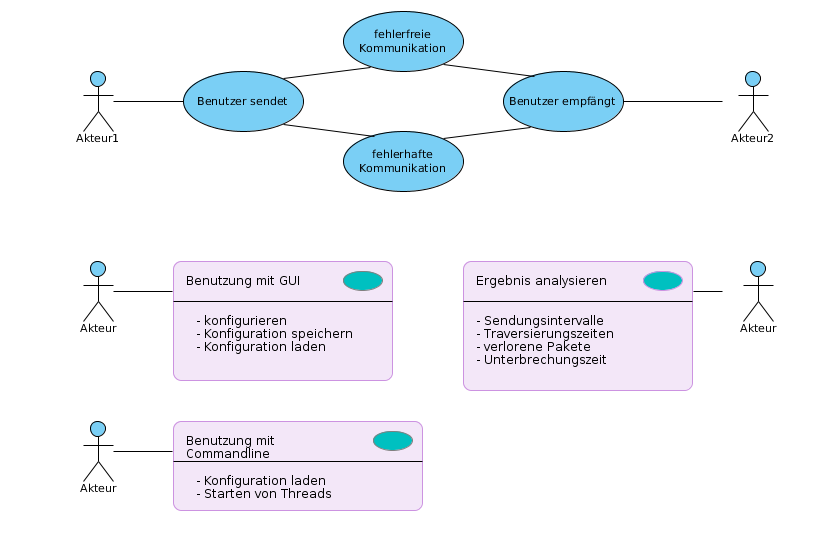
\includegraphics[width=15cm]{images/UseCasesUML.png}
\label{img:usecasesuml}
\caption{Anwendungsfälle}
\end{figure}

\clearpage

\paragraph{/UC10/} Benutzung mit GUI\newline
\texttt{Ziel:} Benutzung des Multicast Test Tools mit grafischem
Userinterface\newline \texttt{Akteure:} Akteur\newline
\texttt{Auslösendes Ereignis:} Akteur startet Programm\newline
\texttt{Beschreibung:}
\begin{itemize}
 \item[-] Starten des Multicast Test Tools mit GUI
 \item[-] Konfiguration des Multicast Test Tools
 \item[-] Speichern einer Konfiguration in Datei
 \item[-] Laden einer Konfiguration aus Datei
\end{itemize}
\texttt{Alternativen:}
\begin{itemize}
 \item[-] Starten des Multicast Test Tools via Commandline
\end{itemize}
\texttt{Testbarkeit:} Starten des Programms


\paragraph{/UC20/} Benutzung via Commandline\newline
\texttt{Ziel:} Benutzung des Multicast Test Tools via Commandline\newline
\texttt{Akteure:} Akteur\newline
\texttt{Auslösendes Ereignis:} Akteur startet Programm\newline
\texttt{Beschreibung:}
\begin{itemize}
 \item[-] Starten des Multicast Test Tools via Commandline
 \item[-] Laden einer Konfiguration von Datei
 \item[-] Starten von Threads
\end{itemize}
\texttt{Alternativen:}
\begin{itemize}
 \item[-] Starten des Multicast Test Tools mit GUI
\end{itemize}
\texttt{Testbarkeit:} Starten des Programms


\paragraph{/UC30/} Benutzer sendet/Benutzer empfängt\newline
\texttt{Ziel:} Testen der Kommunikationsfähigkeit des Netzwerks
\texttt{Akteure:} Akteur1, Akteur2\newline
\texttt{Auslösendes Ereignis:} Starten des Sende- und des
Empfangsvorgangs\newline 
\texttt{Beschreibung:}
\begin{itemize}
 \item[-] Akteur1 sendet Pakete\
 \item[-] Akteur2 versucht Pakete zu empfangen
 \item[-]Kommunikation funktioniert fehlerfrei
\end{itemize}
\texttt{Alternativen:}
\begin{itemize}
  \item[-] Kommunikation ist fehlerhaft, d.h. einige oder alle Pakete gehen
  verloren
\end{itemize}
\texttt{Testbarkeit:} Senden von Paketen zur Überprüfung und Analysieren der
Ergebnisse


\paragraph{/UC40/} Ergebnis analysieren\newline
\texttt{Ziel:} Untersuchung des Netzwerkverhaltens\newline
\texttt{Akteure:} Akteur\newline
\texttt{Auslösendes Ereignis:} Anzeige der Ergebnisse durch das
Multicast Test Tool\newline
\texttt{Beschreibung:}
\begin{itemize}
  \item[-] Analyse der Sendungsintervalle
  \item[-] Analyse der Traversierungszeiten
  \item[-] Analyse der Anzahl der verlorenen Pakete
  \item[-] Analyse der Unterbrechungszeit
\end{itemize}
\texttt{Alternativen:} -\newline
\texttt{Testbarkeit:} Test noch mal durchführen\newline

\clearpage

\section{Verpflichtende Anforderungen}
\label{sec:mandatory}

%TODO Beschreibung konkretisieren

\subsection{Statik}
\label{sec:statik}

\paragraph{/VA0100/ (/LVA0100/)} Multicast-Sendefähigkeit\\
\texttt{Beschreibung:} Das System muss neue IP-Multicast-Gruppen öffnen und
Testströme von UDP-Paketen beliebiger Größe (bis zur Jumbo-Paket-Grenze von
9000bytes) auf beliebigen Ports in Millisekunden-Intervallen versenden können.\\
\texttt{Anforderungsschicht:} Statik/Dynamik\\
\texttt{Priorität:} sehr hoch\\
\texttt{Stabilität:} fest\\
\texttt{Aufwand:} 2 Personentage\\
\texttt{Entwicklungsrisiko:} hoch\\
\texttt{Version und "Anderungsbeschreibung:}

\paragraph{/VA0200/ (/LVA0200/)} Multicast-Empfangsfähigkeit\\
\texttt{Beschreibung:} Das System muss bestehende Multicast-Gruppen
per IGMP abonnieren und Testströme von UDP-Paketen auf beliebigen Ports in
Millisekunden-Intervallen empfangen und deren Eingang protokollieren können.\\
\texttt{Anforderungsschicht:} Statik/Dynamik\\
\texttt{Priorität:} sehr hoch\\
\texttt{Stabilität:} fest\\
\texttt{Aufwand:} 2 Personentage\\
\texttt{Entwicklungsrisiko:} hoch\\
\texttt{Version und "Anderungsbeschreibung:}

\paragraph{/VA0300/ (/LVA0400/)} Gleichzeitigkeit\\
\texttt{Beschreibung:} Das System muss auf einem handelsüblichen Rechner
mindestens 30 Datenströme gleichzeitig senden und empfangen können.\\
\texttt{Anforderungsschicht:}Statik/Dynamik\\
\texttt{Priorität:} hoch\\
\texttt{Stabilität:} fest\\
\texttt{Aufwand:} 2 Personentage\\
\texttt{Entwicklungsrisiko:} hoch\\
\texttt{Version und "Anderungsbeschreibung:}

\paragraph{/VA0400/ (/LVA0500/)} Kompatibilität\\
\texttt{Beschreibung:} Das System muss auf Empfangsseite
mit den Datenströmen des Multicast Test Tools der Hirschmann Automation GmbH
kompatibel sein.\\
\texttt{Anforderungsschicht:} Statik\\
\texttt{Priorität:} hoch\\
\texttt{Stabilität:} gefestigt\\
\texttt{Aufwand:} 3 Personentage\\
\texttt{Entwicklungsrisiko:} mittel\\
\texttt{Version und "Anderungsbeschreibung:}

\paragraph{/VA0500/ (/LVA0600/)} Konfigurierbarkeit\\
\texttt{Beschreibung:} Die Sendekomponente des System muss in folgenden
Punkten konfigurierbar sein: Paketgröße (einschließlich Jumbo-Pakete),
Paket-Senderate, Time-to-live (TTL), Multicast-Gruppe, Port, Nutzdaten
(Zeichenkette), Paketformat\\
\texttt{Anforderungsschicht:} Statik\\
\texttt{Priorität:} hoch\\
\texttt{Stabilität:} gefestigt\\
\texttt{Aufwand:} 2 Personentage\\
\texttt{Entwicklungsrisiko:} hoch\\
\texttt{Version und "Anderungsbeschreibung:}

\paragraph{/VA0600/ (/LVA0800/)} Konfigurationsdatei\\
\texttt{Beschreibung:} Das System muss die Einstellungen zu allen gebotenen
Funktionalitäten in einer Konfigurationsdatei persistieren und aus dieser
wiederherstellen können. Die Konfigurationsdatei soll im XML-Format vorliegen
und syntaktisch leicht verständlich sein, damit der Benutzer sie auch per Hand
erstellen oder ändern kann.\\
\texttt{Anforderungsschicht:} Statik\\
\texttt{Priorität:} hoch\\
\texttt{Stabilität:} gefestigt\\
\texttt{Aufwand:} 3 Personentage\\
\texttt{Entwicklungsrisiko:} mittel\\
\texttt{Version und "Anderungsbeschreibung:}

\paragraph{/VA0700/ (/LVA0900/)} Grafische Nutzeroberfläche\\
\texttt{Beschreibung:} Das System muss sowohl unter Linux, als auch unter
Windows eine einheitliche Benutzeroberfläche bieten, die den Zugriff auf alle Funktionen
des Programms ermöglicht.\\
\texttt{Anforderungsschicht:} Statik\\
\texttt{Priorität:} mittel\\
\texttt{Stabilität:} fest\\
\texttt{Aufwand:} 14 Personentage\\
\texttt{Entwicklungsrisiko:} mittel\\
\texttt{Version und "Anderungsbeschreibung:}

\paragraph{/VA0800/ (/LVA1000/)} Zusammenfassung von Sende- und
Empfangsfunktionalität\\
\texttt{Beschreibung:} Das System muss Sende- und Empfangsfunktionalität
unter derart vereinigen, dass beide Funktionalitäten gemeinsam verteilbar und
steuerbar sind.\\
\texttt{Anforderungsschicht:}
Statik\\ \texttt{Priorität:} mittel\\
\texttt{Stabilität:} fest\\
\texttt{Aufwand:}\\
\texttt{Entwicklungsrisiko:} mittel\\
\texttt{Version und "Anderungsbeschreibung:}

\paragraph{/VA0900/ (/LVA1300/)} Textbasierte Nutzeroberfläche\\
\texttt{Beschreibung:} Das System muss dem Anwender mit einer konsolenbasierten
Nutzerschnittstelle die Steuerung aller Programmfunktionen per
Konfigurationsdatei oder Parametern ermöglichen. Die Konsolenschnittstelle muss
intuitiv in Skripten eingebunden werden können. Die Ergebnisse müssen in einfach weiterzuverarbeiten
Logdateien festgehalten werden.\\
\texttt{Anforderungsschicht:} Statik\\
\texttt{Priorität:} mittel\\
\texttt{Stabilität:} fest\\
\texttt{Aufwand:} 14 Personentage\\
\texttt{Entwicklungsrisiko:} mittel\\
\texttt{Version und "Anderungsbeschreibung:}

\subsection{Dynamik}
\label{sec:dynamik}

\paragraph{/VA1000/ (/LVA0700/)} Sendestatistik\\
\texttt{Beschreibung:} Die Sendekomponente des System muss laufende
Informationen zu folgenden Punkten ausgeben: Anzahl der gesendeten Pakete
(gesamt, pro MC-Gruppe), Paketraten (gesamt, pro MC-Gruppe), per Zufall
generierte Sender-Identifikationsnummer\\
\texttt{Anforderungsschicht:} Dynamik\\
\texttt{Priorität:} hoch\\
\texttt{Stabilität:} gefestigt\\
\texttt{Aufwand:} 1 Personentage\\
\texttt{Entwicklungsrisiko:} mittel\\
\texttt{Version und "Anderungsbeschreibung:}

\paragraph{/VA1100/ (/LVA1100/)} Darstellung der Sendeströme\\
\texttt{Beschreibung:} Ausgehende Multicast-Datenströme müssen mit ihren
Parametern in einer Liste angezeigt werden. Die Ströme müssen in der Liste
direkt per Mausklick aktivierbar und deaktivierbar sein. Die Liste soll es dem
Anwender außerdem erlauben, die Parameter mehrerer Sendeströme gleichzeitig zu
bearbeiten.\\
\texttt{Anforderungsschicht:} Dynamik/Statik\\
\texttt{Priorität:} mittel\\
\texttt{Stabilität:} volatil\\
\texttt{Aufwand:}\\
\texttt{Entwicklungsrisiko:} mittel\\
\texttt{Version und "Anderungsbeschreibung:}

\paragraph{/VA1200/ (/LVA1200/)} Messwertanzeige\\
\texttt{Beschreibung:} Die grafische Oberfläche muss die nach /VA1300/
ermittelten Messwerte als dem jeweiligen Datenstrom eindeutig zugehörig
darstellen.\\
\texttt{Anforderungsschicht:} Dynamik/Statik\\
\texttt{Priorität:} mittel\\
\texttt{Stabilität:} fest\\
\texttt{Aufwand:} 3 Personentage\\
\texttt{Entwicklungsrisiko:} mittel\\
\texttt{Version und "Anderungsbeschreibung:}

\subsection{Logik}
\label{sec:logik}

\paragraph{/VA1300/ (/LVA0300/)} Datenauswertung\\
\texttt{Beschreibung:} Die Empfangskomponente des Systems muss Daten bezüglich
folgender Punkte bereitstellen: Anzahl und Dauer von Unterbrechungen, Paketrate
(gesamt, pro MC-Gruppe), Anzahl empfangener Pakete (gesamt, pro MC-Gruppe),
Anzahl verlorener Pakete (gesamt, pro MC-Gruppe), Empfang fehlerhafter Pakete\\
\texttt{Anforderungsschicht:} Logik\\
\texttt{Priorität:} hoch\\
\texttt{Stabilität:} gefestigt\\
\texttt{Aufwand:} 3 Personentage\\
\texttt{Entwicklungsrisiko:} hoch\\
\texttt{Version und "Anderungsbeschreibung:}

\section{Optionale Anforderungen}
\label{sec:optional}


\paragraph{/OA0100/ (/LOA0100/)} IPV6 Unterstützung\\
\texttt{Beschreibung:} Das Programm soll in Zukunft fähig sein Multicasts in
IPV6 Netzwerken testen zu können.\\
\texttt{Anforderungsschicht:} Statik\\ 
%Querbez"uge: keine \\
\texttt{Abnahmekriterien:} Das Programm in einer IPV6 Umgebung testen.\\
\texttt{Priorit"at:} Niedrig\\
\texttt{Stabilit"at:} Fest\\
\texttt{Aufwand:} 5 Personentage\\
\texttt{Entwicklungsrisiko:} Mittel\\
\texttt{Version und "Anderungsbeschreibung:}\newline

\paragraph{/OA0200/ (/LOA0200/)} NTP Zeitsynchronisierung\\
\texttt{Beschreibung:} Verschiedene Sender und Empfänger sollen in Zukunft
ihre Zeit über NTP synchronisieren um die Traversierungszeit von Paketen
ermitteln zu können.\\ 
\texttt{Anforderungsschicht:} Statik\\ 
\texttt{Abnahmekriterien:} Die Zeitsynchronisierung in den Logdateien
nachvollziehen.\\ 
\texttt{Priorit"at:} Niedrig\\
\texttt{Stabilit"at:} Volatil\\
\texttt{Aufwand:} 2 Personentage\\
\texttt{Entwicklungsrisiko:} Mittel\\
\texttt{Version und "Anderungsbeschreibung:}

\paragraph{/OA0300/ (/LOA0300/)} Darstellung der Messergebnisse\\
\texttt{Beschreibung:} Die Messergebnisse sollen mithilfe von Farbcodes oder
Grafiken präsentiert werden. Verlorene Pakete und Geschwindigkeitsunterschiede
sollen so auf einen Blick erfassbar gemacht werden.\\
\texttt{Anforderungsschicht:} Statik\\ 
\texttt{Abnahmekriterien:} Durchführen von Messungen und validieren der
generierten Grafiken anhand der ausgegebenen Messwerte.\\ 
\texttt{Priorit"at:} Niedrig\\
\texttt{Stabilit"at:} Volatil\\
\texttt{Aufwand:} 2 Personentage\\
\texttt{Entwicklungsrisiko:} Mittel\\
\texttt{Version und "Anderungsbeschreibung:}

\paragraph{/OA0400/ (/LOA0400/)} Nutzdatenübertragung\\
\texttt{Beschreibung:} In Zukunft soll es möglich sein Nutzdaten in den
UDP-Datagrammen zu übertragen.\\
\texttt{Anforderungsschicht:} Statik\\ 
\texttt{Abnahmekriterien:} Übertragung von Nutzdaten und validieren der Daten
nach der Übertragung mit Hilfe eines Hash-Wertes.\\
\texttt{Priorit"at:} Niedrig\\
\texttt{Stabilit"at:} Volatil\\
\texttt{Aufwand:} 1 Personentag\\
\texttt{Entwicklungsrisiko:} Gering\\
\texttt{Version und "Anderungsbeschreibung:}